\documentclass[12pt, a4paper, oneside]{article}
\usepackage{graphicx}
\usepackage{arial}
\renewcommand{\familydefault}{\sfdefault}
\usepackage[T1]{fontenc}
\usepackage[polish]{babel}
\usepackage[utf8]{inputenc}
\usepackage{lmodern}
\usepackage[left=2cm,right=2cm,top=2cm,bottom=2cm]{geometry}
\selectlanguage{polish}

\begin{document}
\pagenumbering{gobble}
\pagenumbering{arabic}
\section{Wstęp}
\indent\indent Złącza światłowodowe pozwalają na łączenie ze sobą kolejnych odcinków światłowodu lub łączenia światłowodów z elementami sieci, jak choćby sprzęgacze. Istnieją fabryczne oraz ręczne metody ich zarabiania. Podczas laboratorium ręcznie zarabia się złącze światłowodowe, które następnie jest szlifowane i poddawane kontroli pod mikroskopem. Zdecydowaną wadą ręcznego zarabiania złączy jest niska jakość wykonana i znacząco większe straty odbiciowe w stosunku do złączy zarabianych fabrycznie. Etapy zarabiania złącza:
\begin{itemize}
\item usunięcie płaszcza światłowodu za pomocą strippera,
\item wyczyszczenie włókna światłowodowego za pomocą płynu z alkoholem,
\item wprowadzenie włókna do ceramicznej ferruli,
\item przyklejenie włókna,
\item ucięcie nadmiaru włókna i wypolerowanie złącza.
\end{itemize}
\section{Przebieg ćwiczenia}
\indent\indent Dwie osoby z grupy odpowiedzialne były za zarobienie złącza SM FC/APC. Główną trudnością na tym etapie ćwiczenia było przełożenie włókna przez otwór w ferruli. Druga część zespołu w tym czasie zajęła się polerowaniem oraz badaniem struktury złącza pod mikroskopem.
\begin{figure}[h]
\centering
\caption{Włókno światłowodowe wystające w nadmiarze z zarobionego złącza}
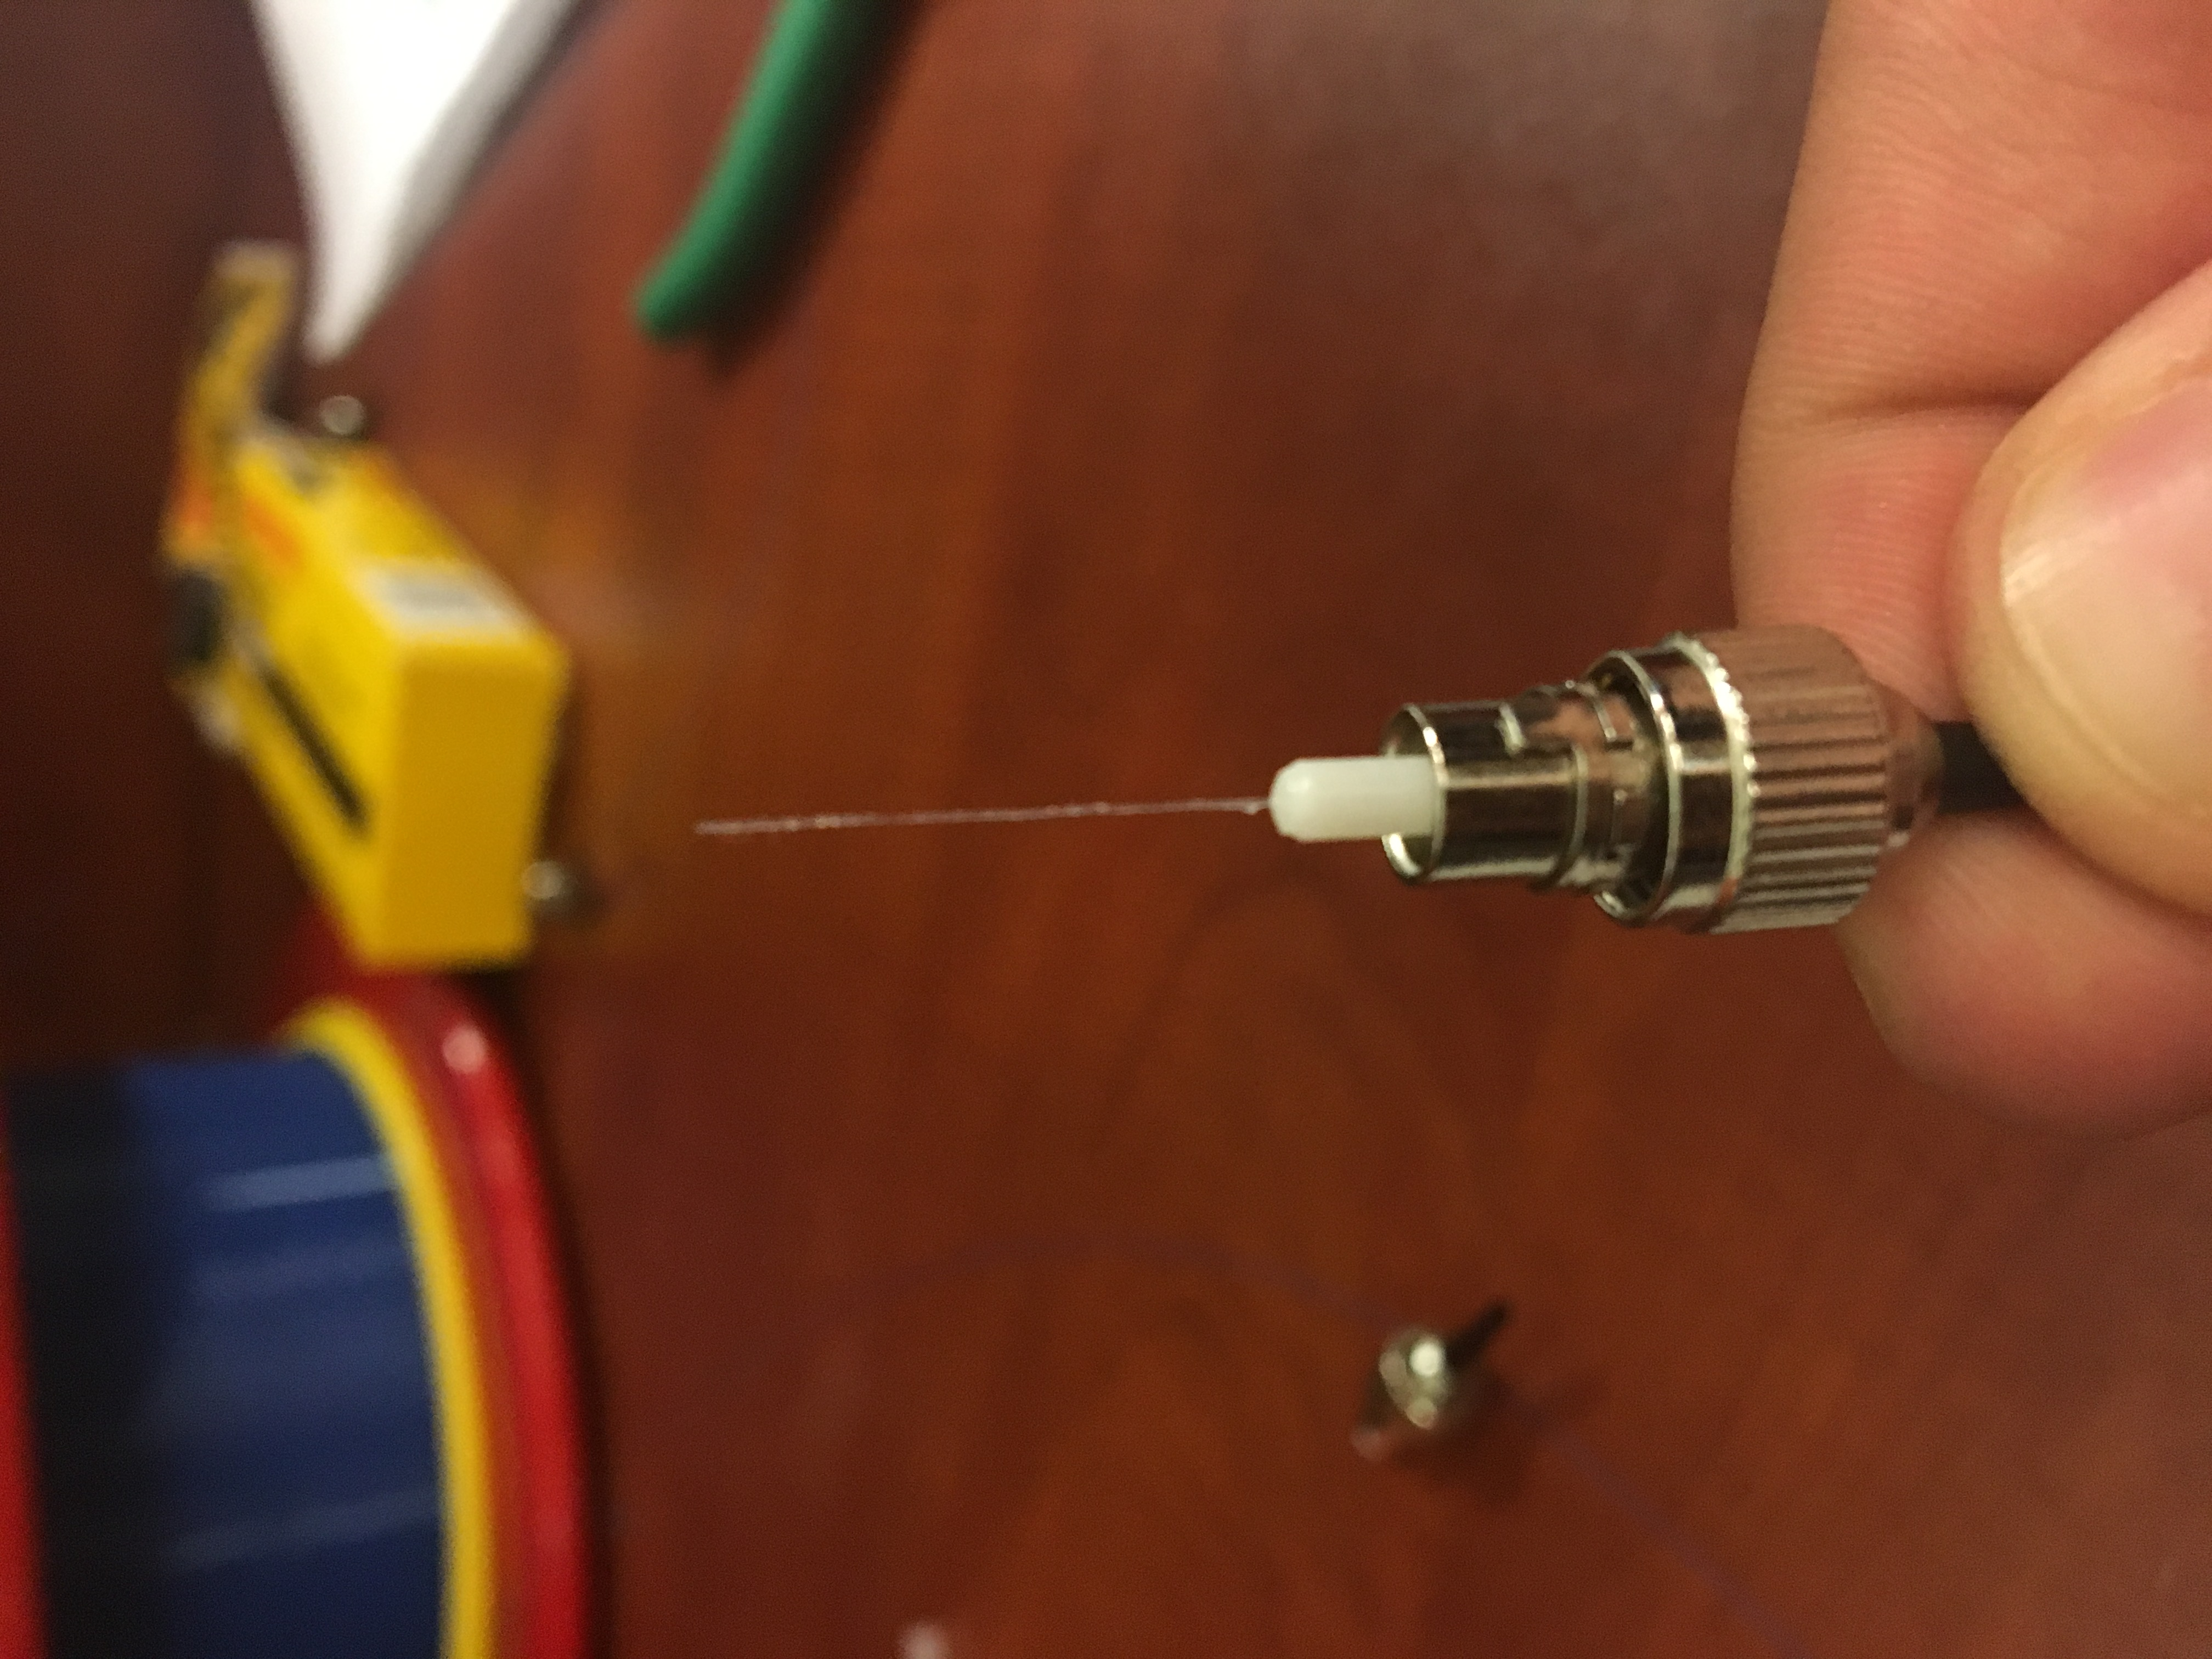
\includegraphics[scale=0.1]{m3.jpg}
\end{figure}
\clearpage
\begin{figure}[t]
\centering
\caption{Celowo zabrudzone złącze światłowodowe}
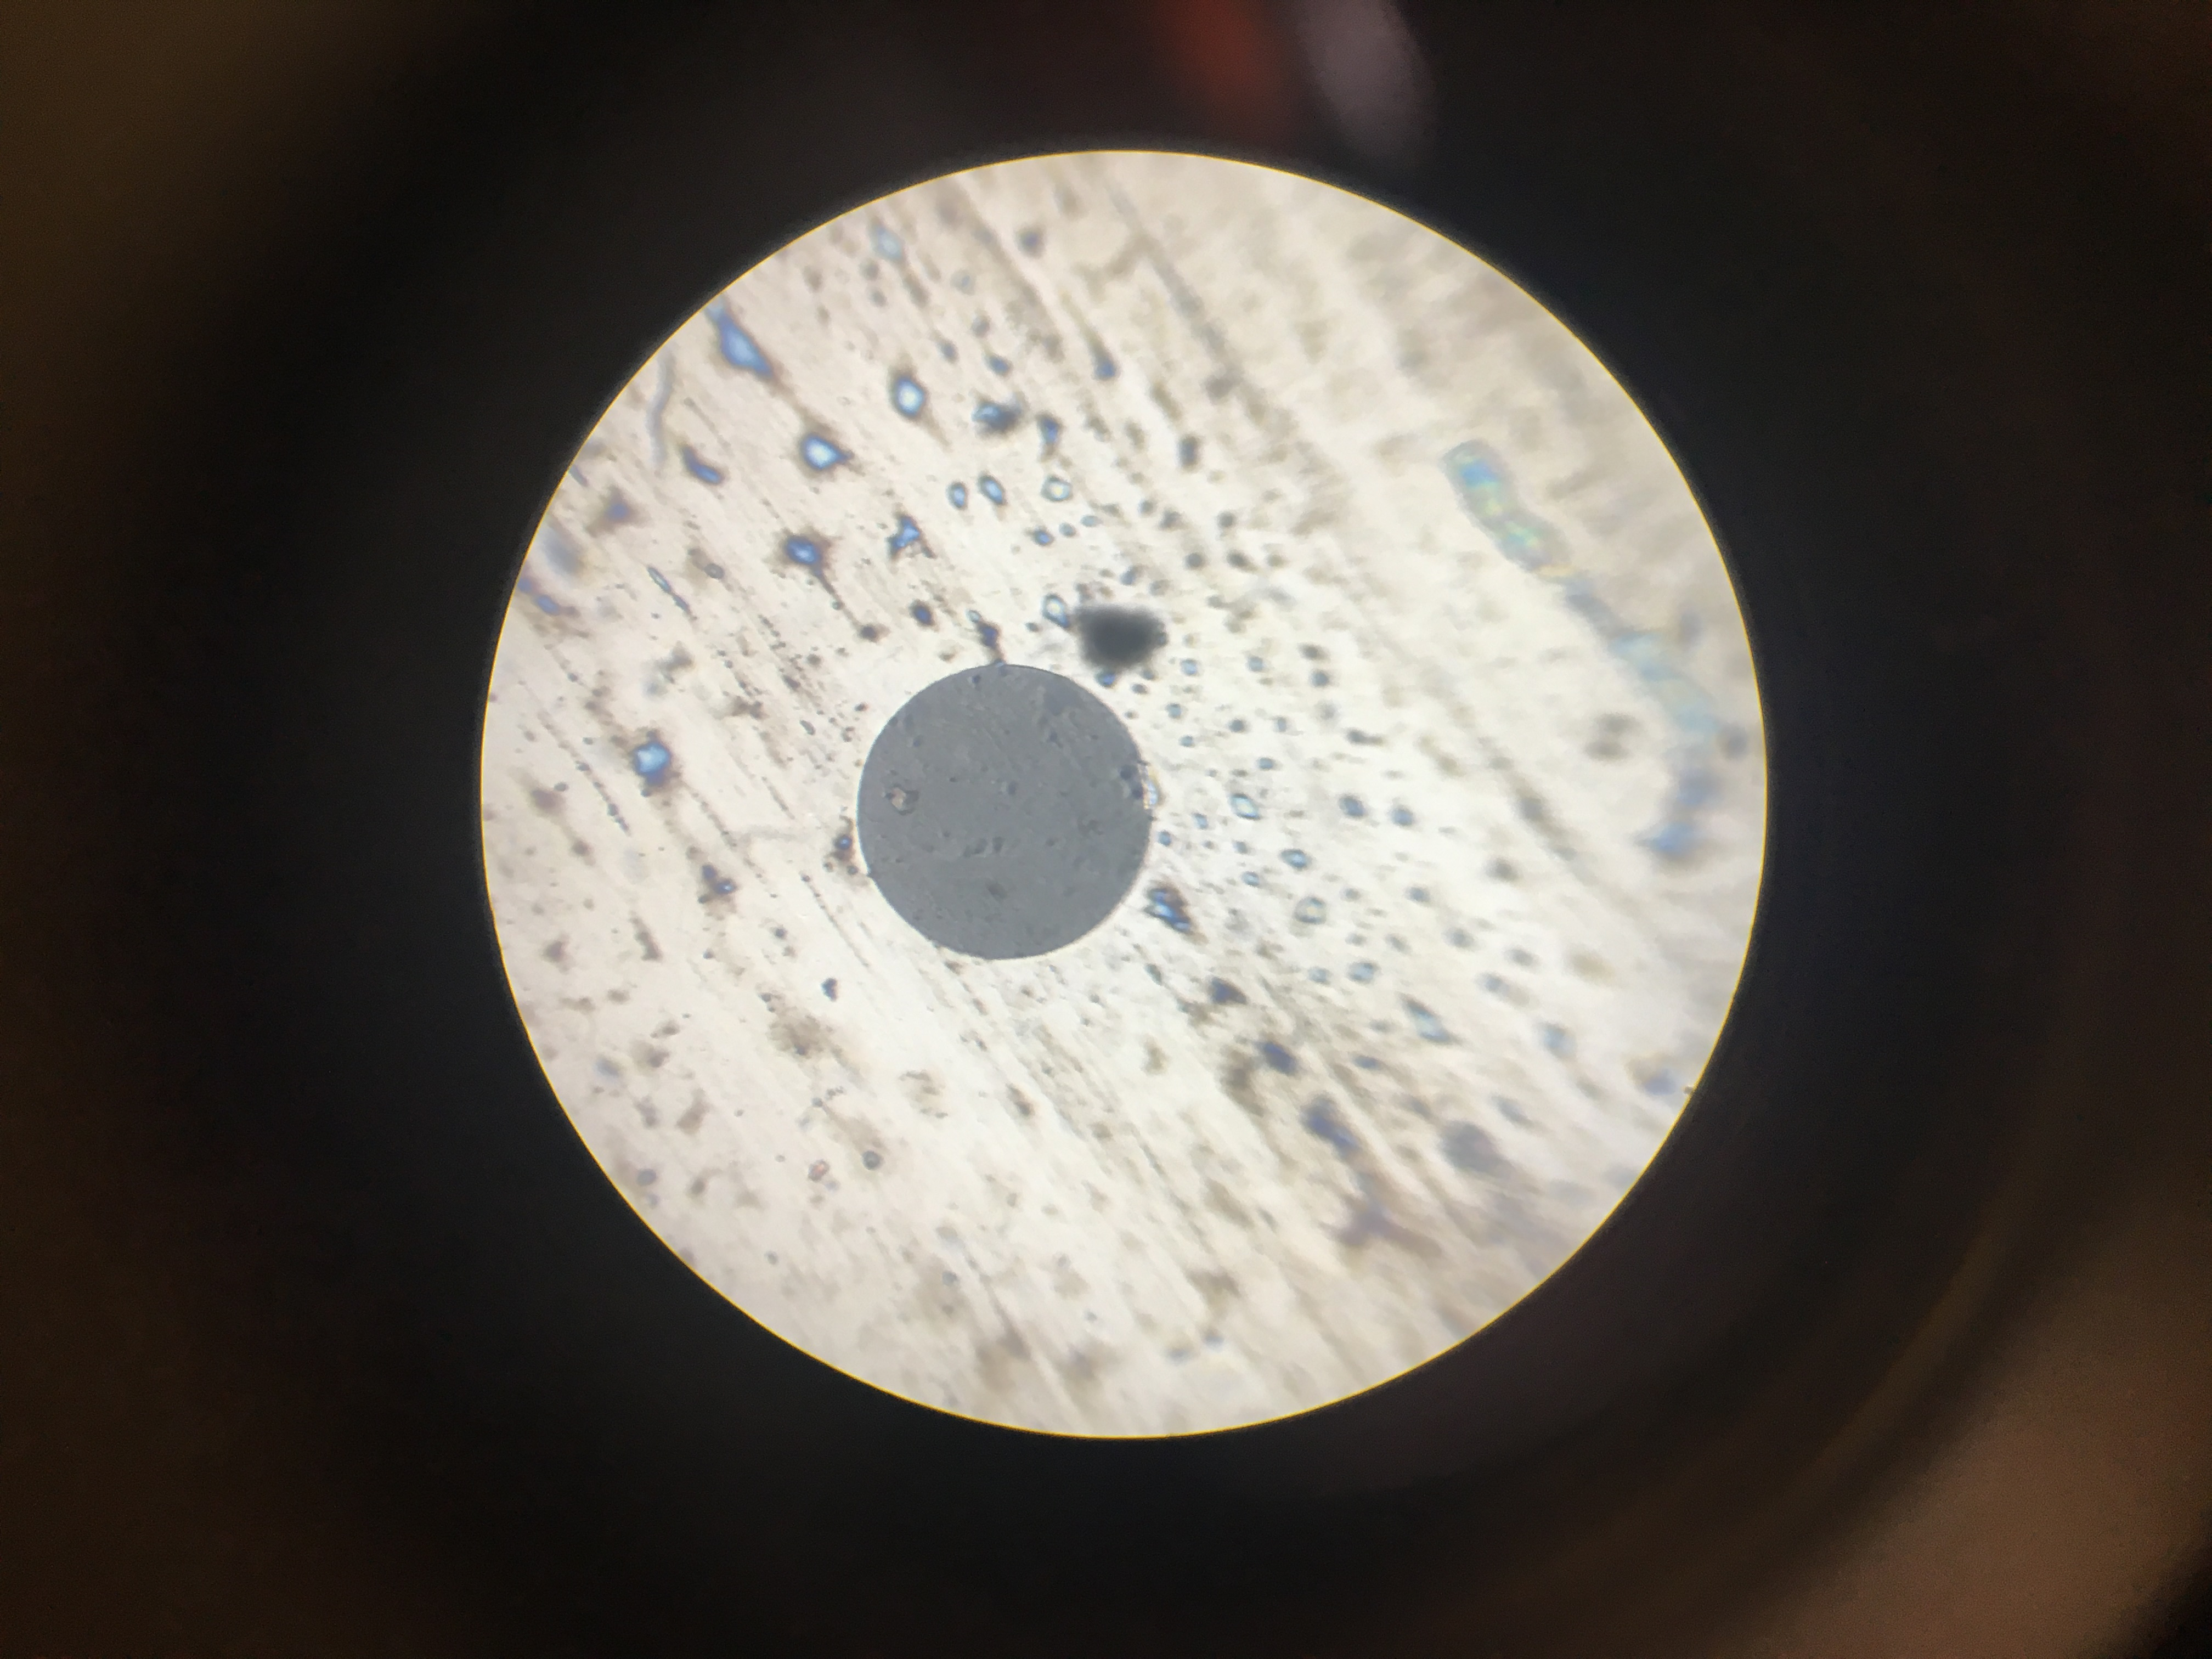
\includegraphics[scale=0.1]{m1.jpg}
\end{figure}
\begin{figure}[b]
\centering
\caption{Złącze z rys. 1 po wyczyszczeniu za pomocą czyścika}
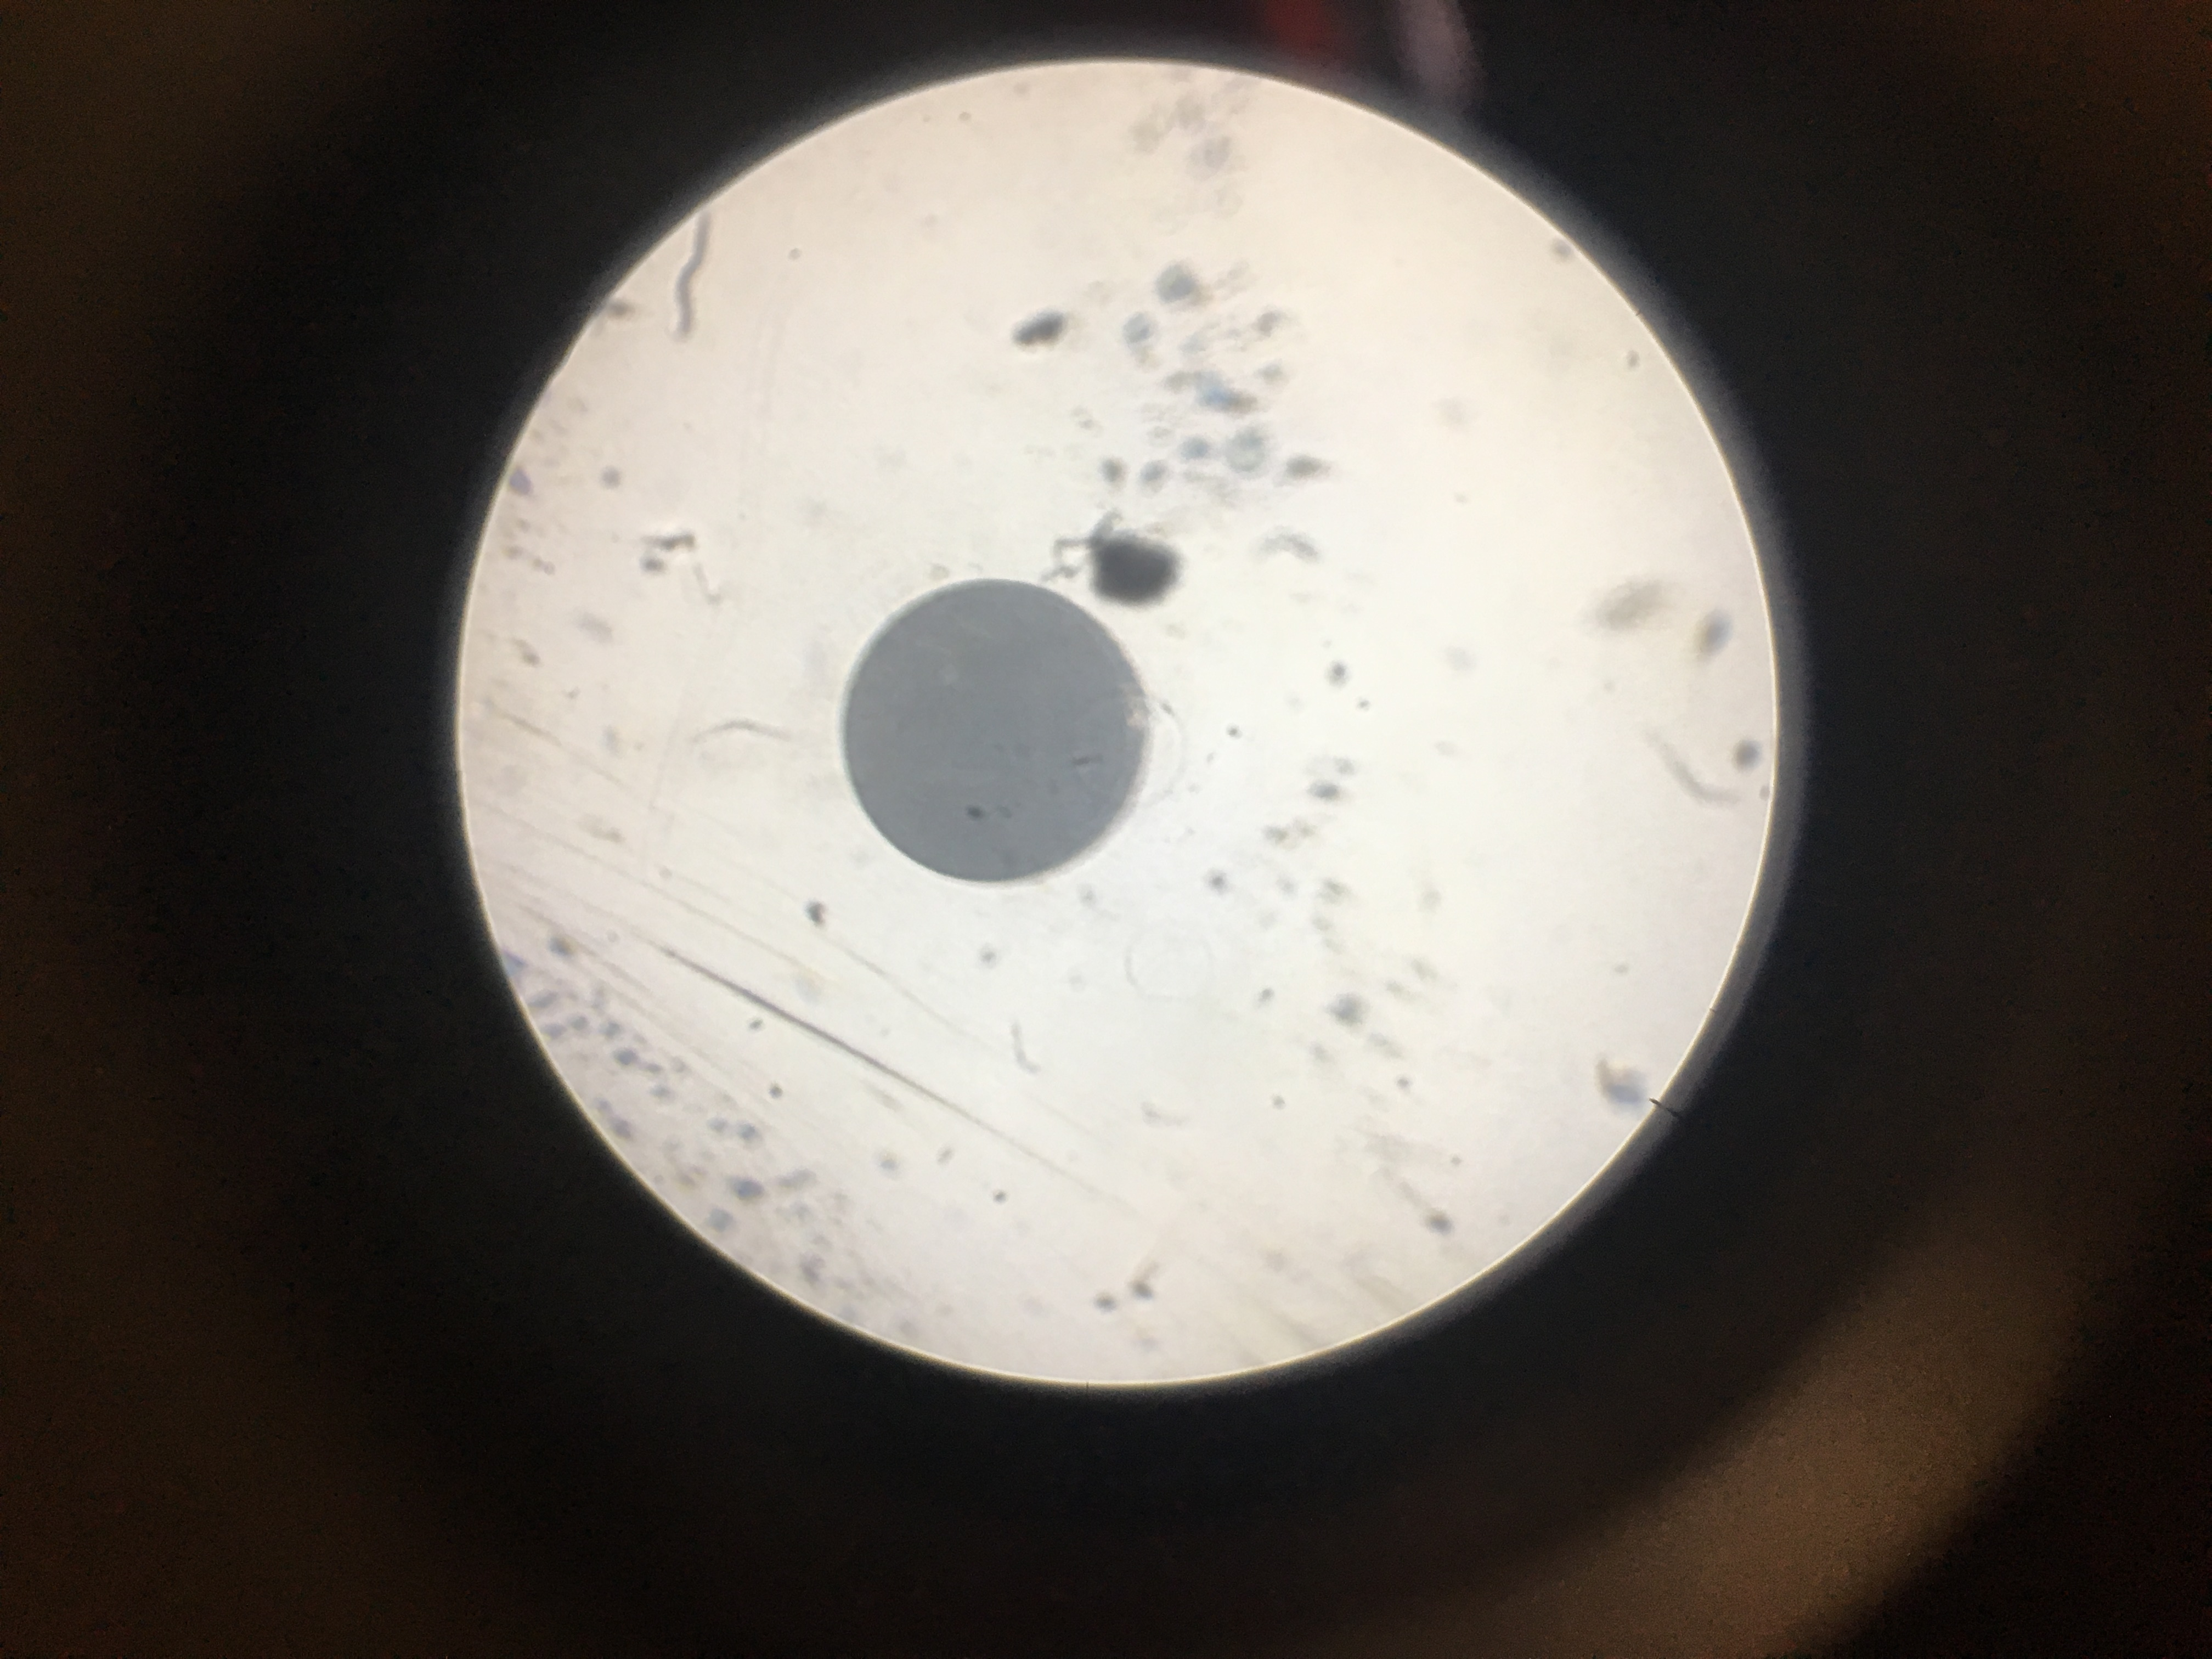
\includegraphics[scale=0.1]{m2.jpg}
\end{figure}
\clearpage
\begin{figure}[t]
\centering
\caption{Przykładowe wypolerowane złącze światłowodu wielomodowego dostępnego na stanowisku laboratoryjnym}
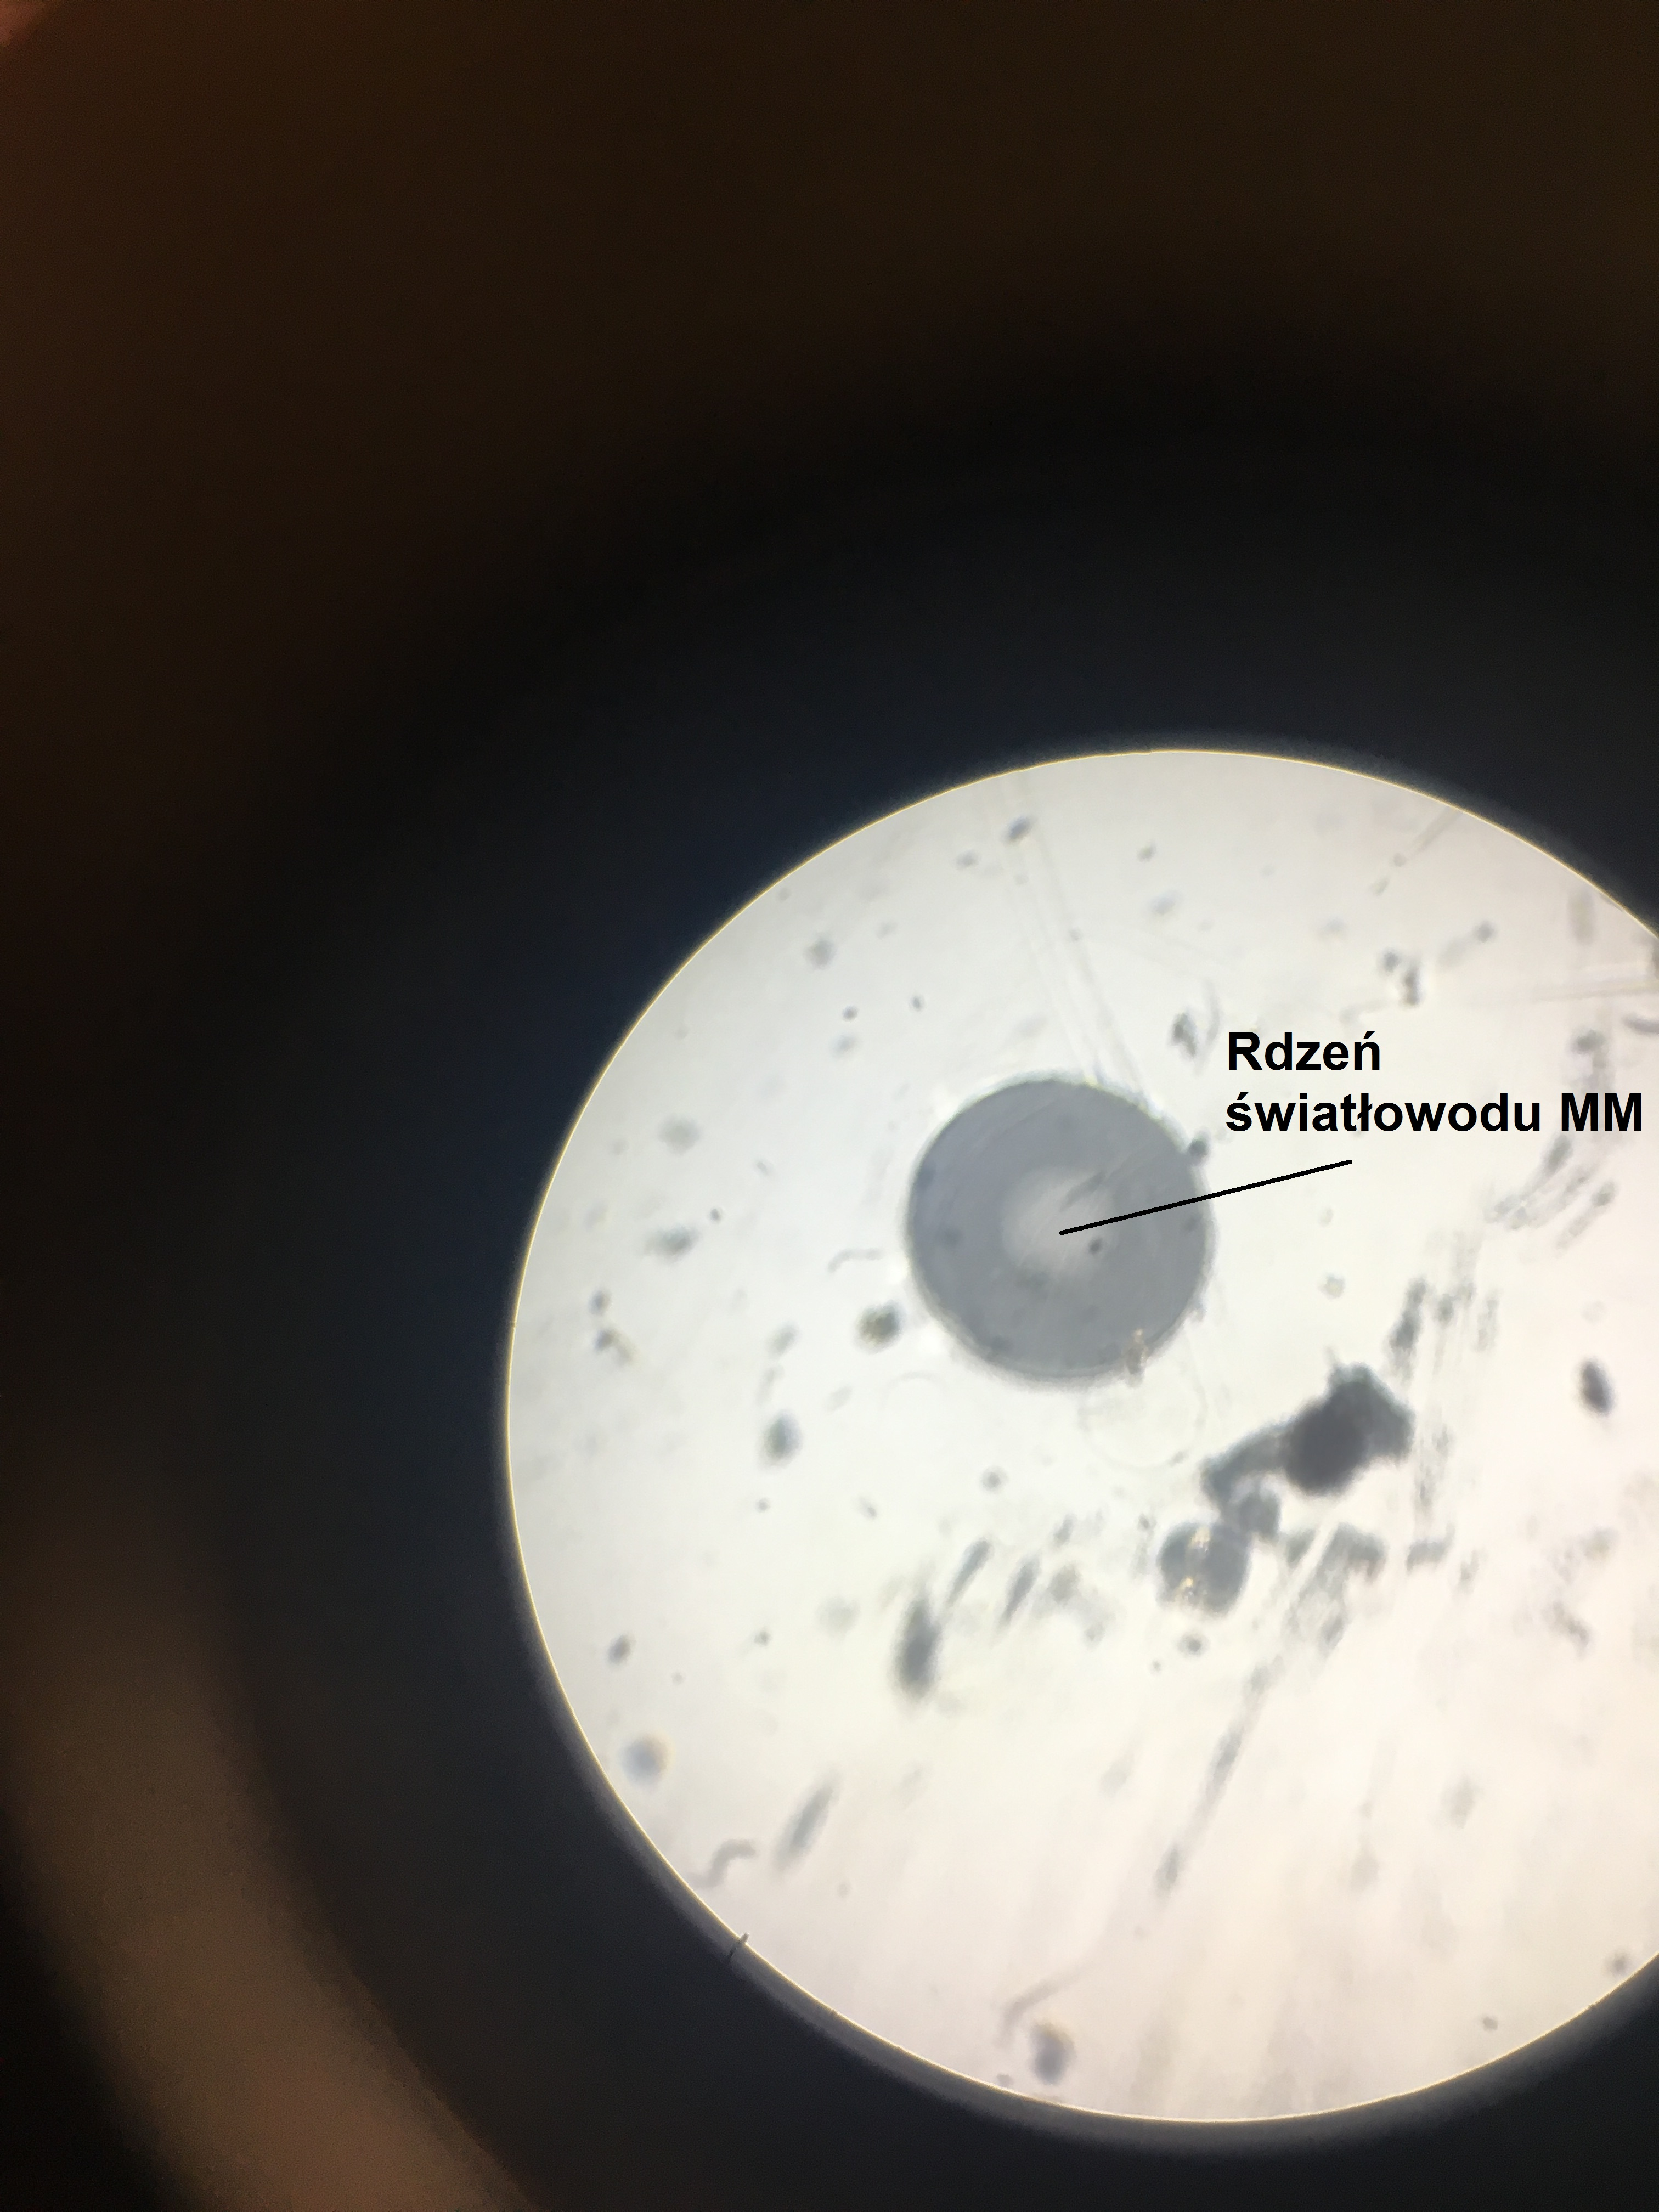
\includegraphics[scale=0.1]{m4.jpg}
\end{figure}
\indent Szlifowanie złącza jest procesem wieloetapowym. Szlifuje się kolejno na różnych powierzchniach. Podczas laboratorium wykorzystane zostały kolejno następujące papiery polerskie:
\begin{itemize}
\item czarny - płyta szklana,
\item żółty - plexi,
\item różowy - plexi.
\end{itemize}
\indent\indent Na każdej warstwie polerskiej wykonuje się około 20 - 30 "ósemek". Po użyciu trzech wyżej wymienionych warstw przeprowadzano kontrolę pod mikroskopem. Proces powtarzano, aż do osiągnięcia zadowalającego efektu - kiedy kolejne powtórzenia procesu nie poprawiały znacząco jakości złącza.
\clearpage
\begin{figure}[t]
\centering
\caption{Mocno zarysowane złącze światłowodowe}
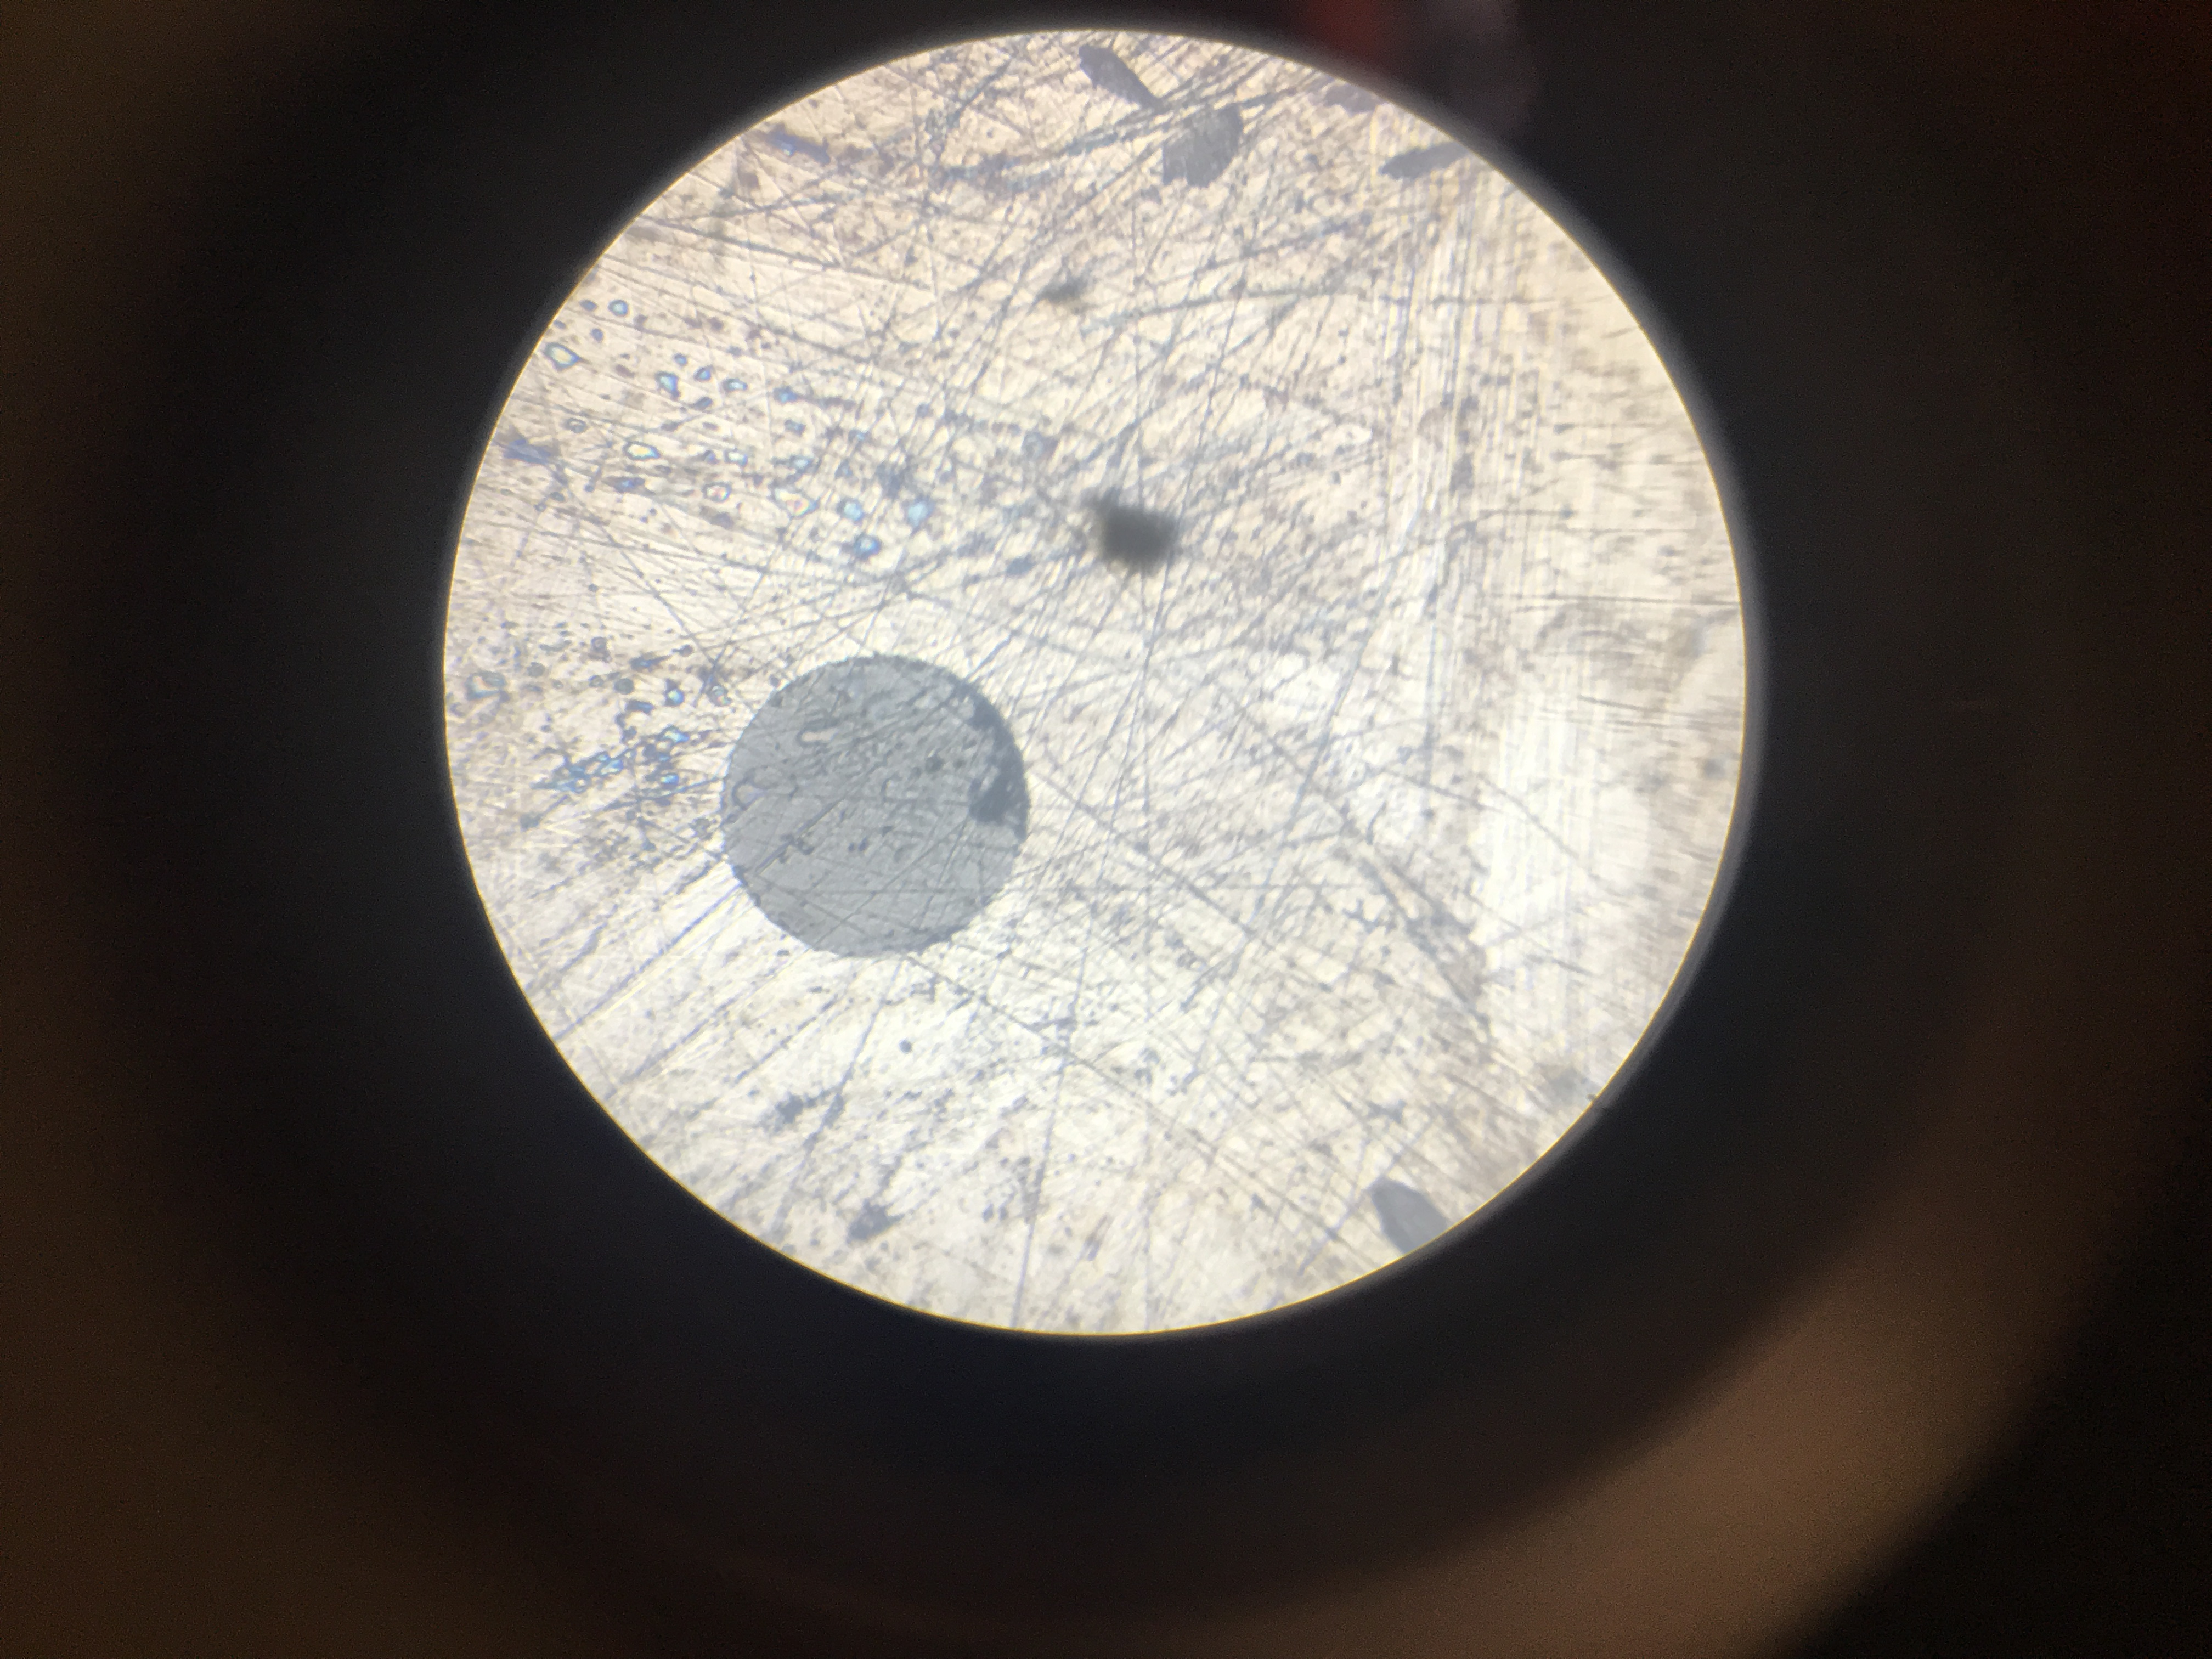
\includegraphics[scale=0.1]{m5.jpg}
\end{figure}
\begin{figure}[b]
\centering
\caption{Złącze światłowodowe po jednym powtórzeniu procesu polerowania}
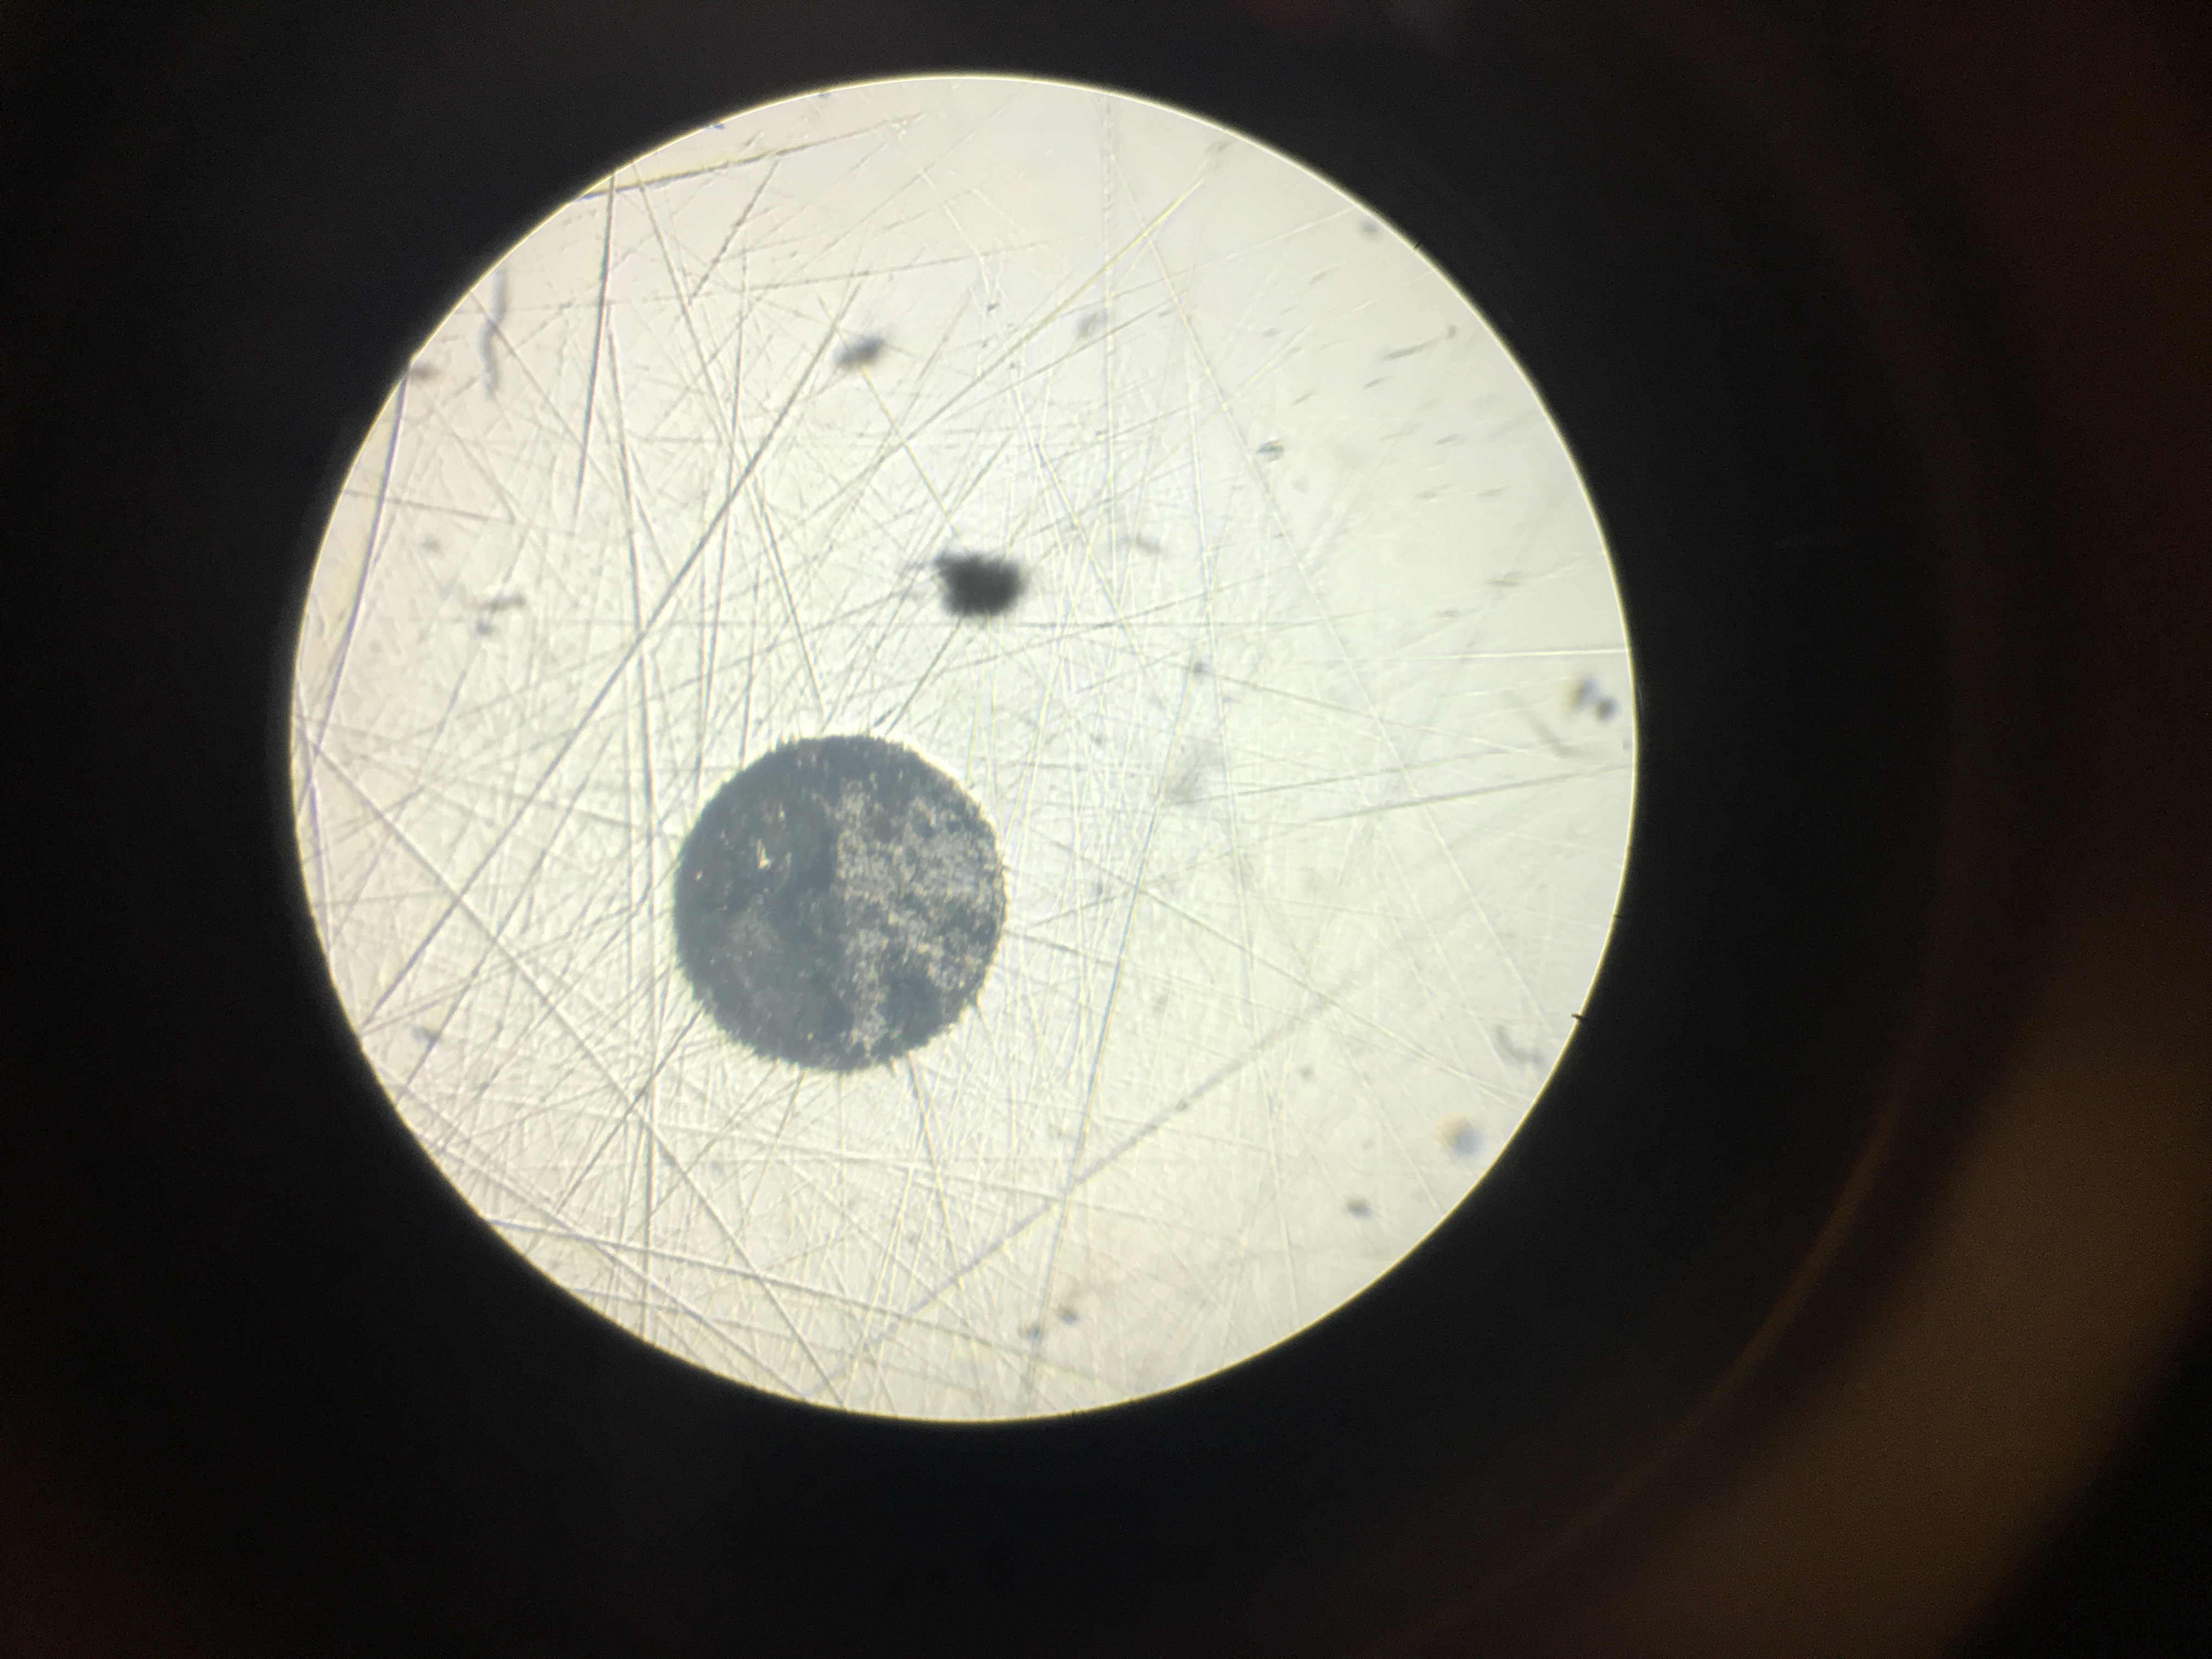
\includegraphics[scale=0.1]{m6.jpg}
\end{figure}
\clearpage
\begin{figure}[t]
\centering
\caption{Złącze światłowodowe po czterech powtórzeniach procesu polerowania}
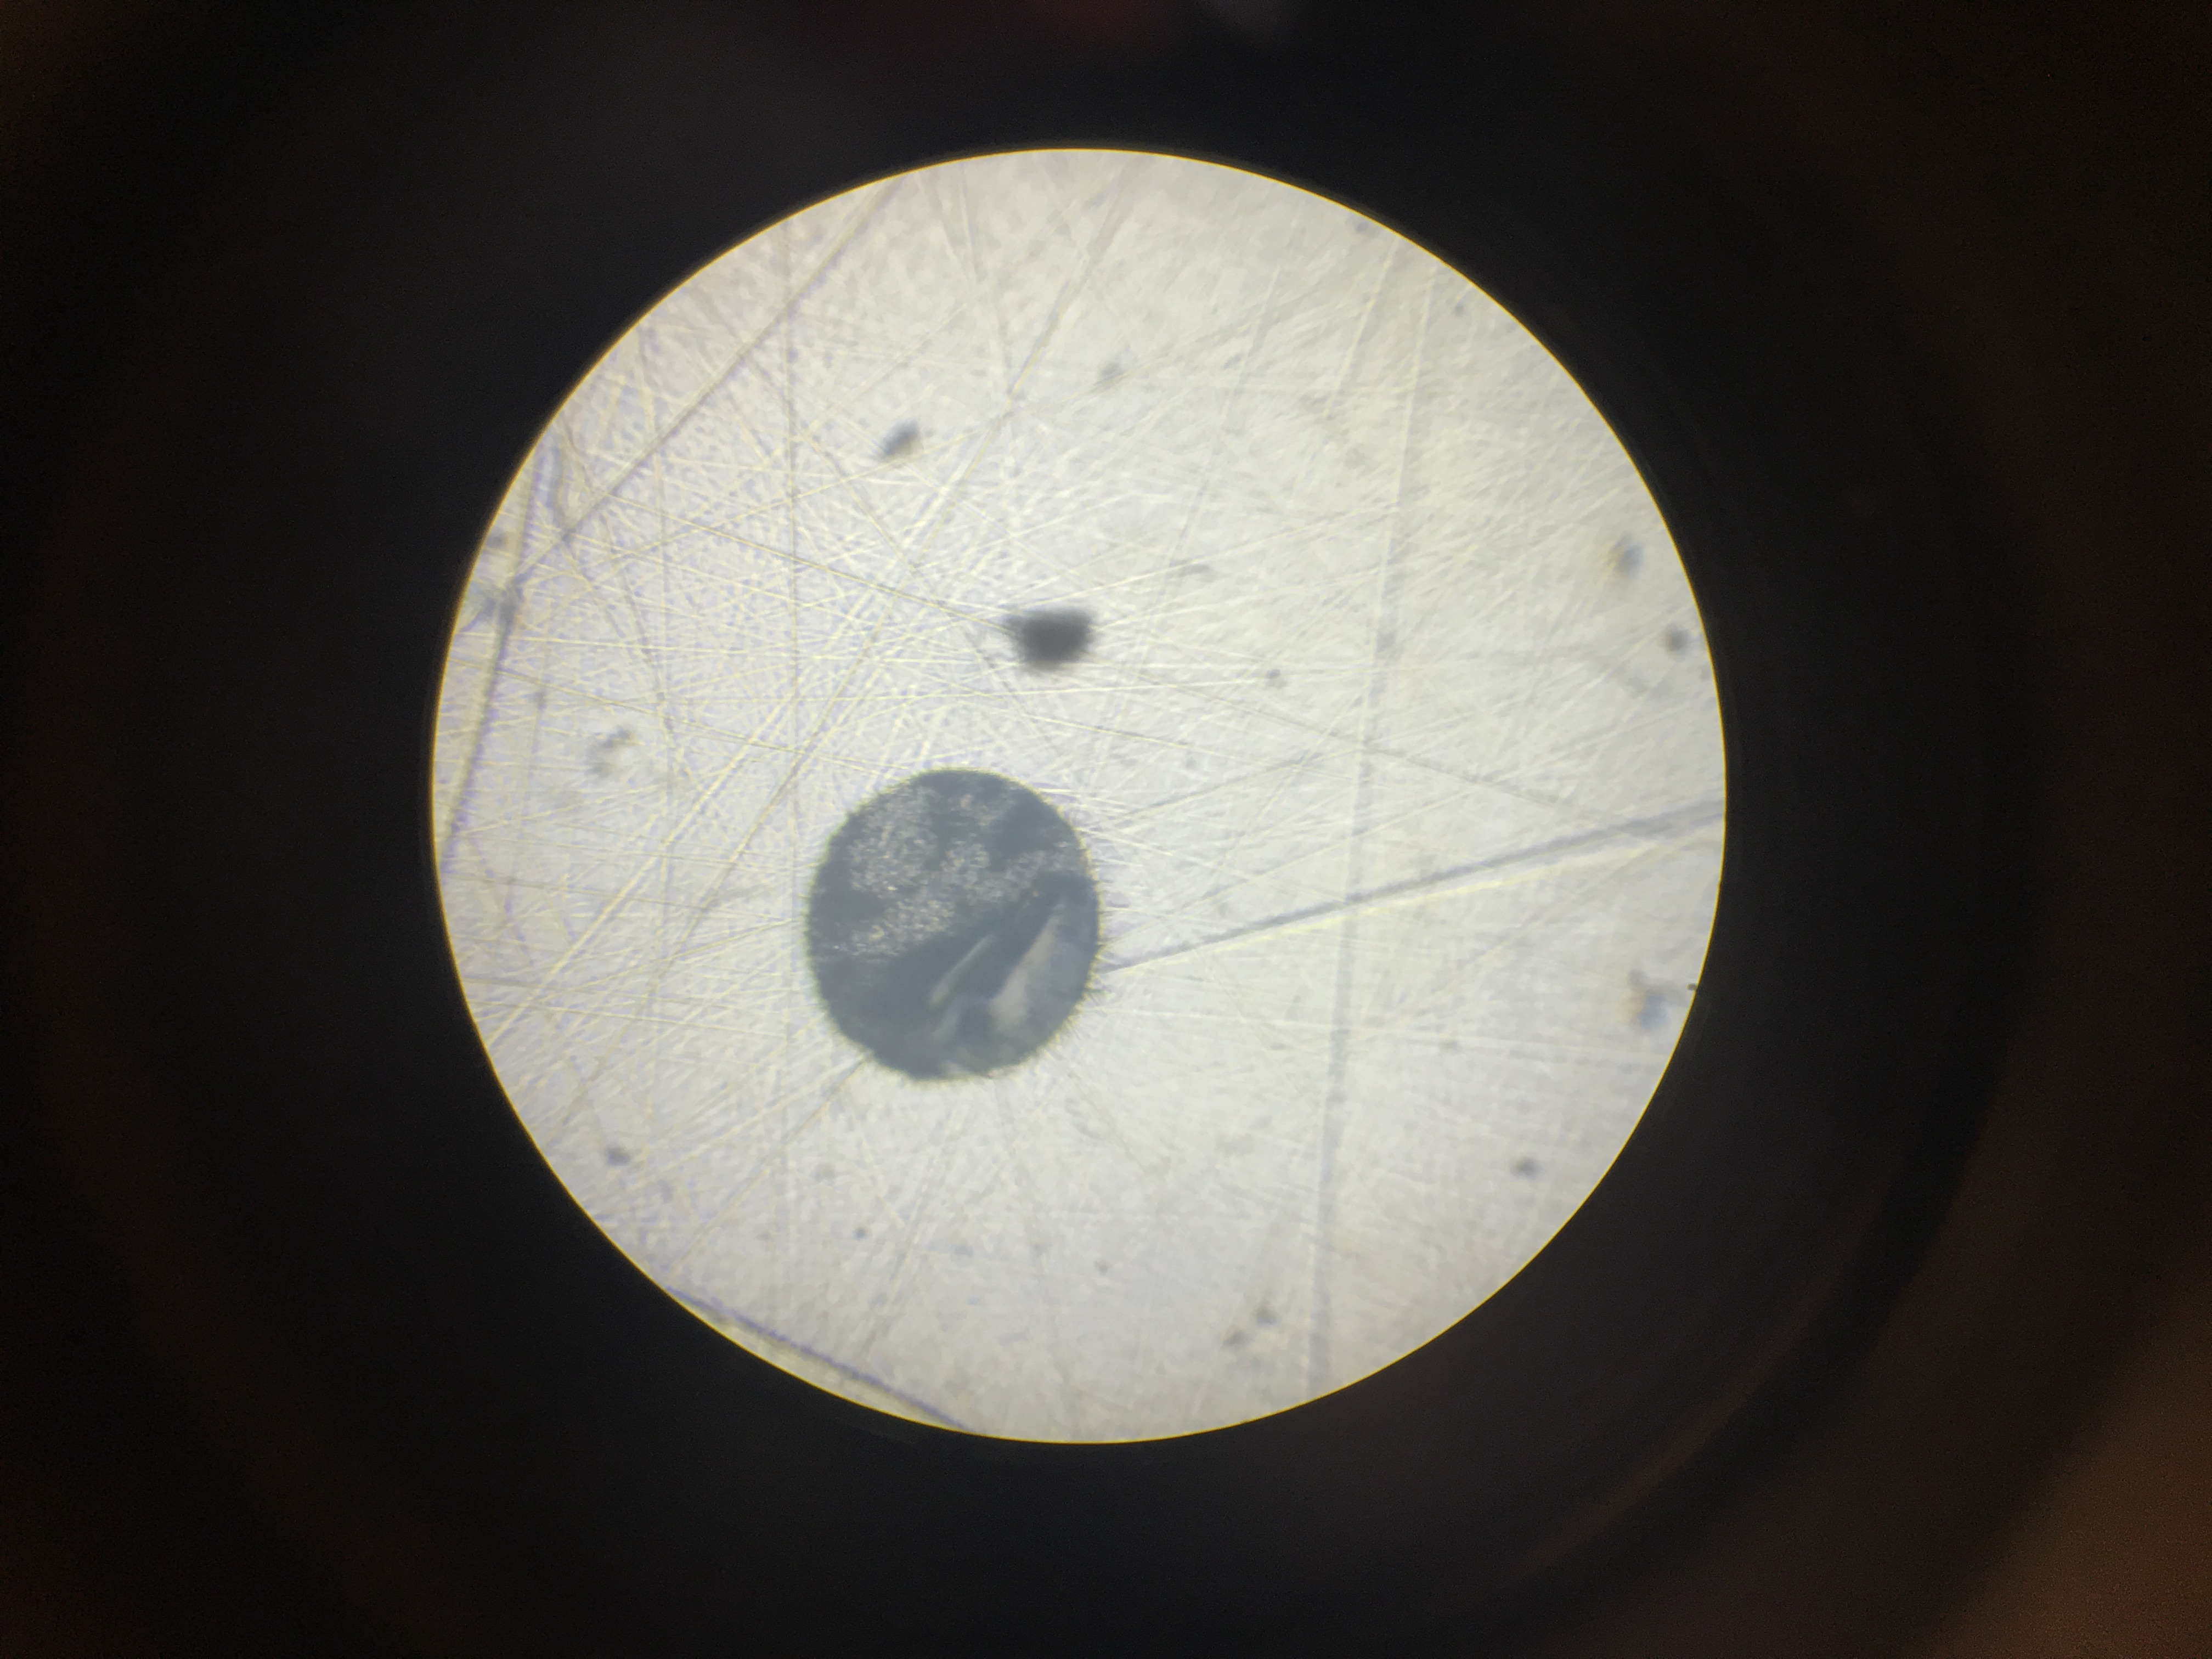
\includegraphics[scale=0.11]{m7.jpg}
\end{figure}
\section{Wnioski}
\begin{itemize}
\item Ręczne zarabianie złączy jest procesem czasochłonnym dla osób początkujących.
\item Zarabianie złączy wymaga zachowania czystości na stanowisku laboratoryjnym, aby przypadkowe zanieczyszczenia nie powodowały dodatkowych strat w złączu.
\item Polerowanie pozwala na zmniejszenie strat odbiciowych w złączu.
\item Podczas obserwacji dla złączy SM niemożliwe było zaobserwowanie rdzenia. Udało się to zrobić dla złącza światłowodu MM. 
\end{itemize}
\end{document}